\documentclass{article}

% Language setting
% Replace `english' with e.g. `spanish' to change the document language
\usepackage[UTF8]{ctex}

% Set page size and margins
% Replace `letterpaper' with `a4paper' for UK/EU standard size
\usepackage[letterpaper,top=2cm,bottom=2cm,left=3cm,right=3cm,marginparwidth=1.75cm]{geometry}

% Useful packages
\usepackage{amsmath}
\usepackage{amsfonts,amssymb}
\usepackage{bm}
\usepackage{graphicx}
\usepackage[colorlinks=true, allcolors=blue]{hyperref}

\title{多元函数入门攻略(上)}
\date{}
\author{Author:洛}

\begin{document}
\maketitle


本文主要讲述多元函数(以2个自变量的函数为例)极限、可微、连续、偏导数和方向导数之间的关系以及做题方法。分为以下5个部分:概述、定义、常见题型、反例、总结。



\tableofcontents

\newpage
\setcounter{page}{1}

\section{概述}
\begin{figure}[!h]
    \centering
    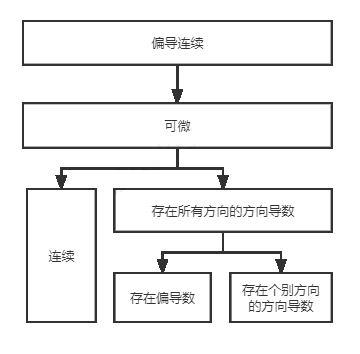
\includegraphics[width=0.5\textwidth]{pic/01.png}
    \caption{关系图}
\end{figure}

上面图中,越往上代表该命题越强,处于上面的结论可以推出处于下面的结论(例如:在某点可微可以推出在这一点连续),处于下面的结论不能推出处于上面的结论(例如:在某点所有方向都存在方向导数不能得到在这一点可微),而同等级的结论之间也不能互推(例如:在某点连续不能推出在这一点存在偏导数)

\textcolor{red}{注:所有性质都是基于某一点处进行讨论,如:在某点连续、在某点可微}


\section{定义}
(我尽量以通俗易懂,从已经学过的一元向多元推广的方式来叙述枯燥无味的定义)

\subsection{极限}
多元函数极限的定义和一元函数类似,在此不多赘述。(其实$\epsilon-\delta$语言描述的严格定义没必要知道)

不过要注意的是,在某一点的极限存在必须从各个方向趋近这个点极限值相等。
比如在一元函数$f(x) = \begin{cases}1 & x  \geq  0\\0 & x < 0\end{cases}$在$x=0$这点没极限,是因为从x轴正方向趋近极限值是1,从x负方向趋近极限值是0,这两个方向趋近于$x=0$这一点极限值不相等,所以在这点没有极限。

同样的推广到二元函数,二元函数只是从一元函数的两个方向变成了趋近某一点的多个方向(无限个)。那么同理,所有方向趋近于某点的极限值必须全部相等,这一点才有极限。

\subsection{连续}
简而言之,函数在某点连续的定义是函数趋近于这一点的极限与这一点的函数值相等,即
\[\lim\limits_{(x,y) \rightarrow (x_0,y_0)} f(x,y)=f(x_0,y_0)\]

那么这个定义隐含的意思是,如果函数趋近于$(x_0,y_0)$的极限不存在(等式左边不存在),或者在$(x_0,y_0)$处没有定义(等式右边不存在),那么函数在$(x_0,y_0)$自然也就不连续了。

\subsection{方向导数}
方向导数即为在某一方向的导数,我们用一个模长为1向量$\mathbf{u}$来表示一个方向。

在一元函数中,f(x)在$x_0$一点沿x正方向的导数的定义是
\[f'(x_0^+) = \lim\limits_{\Delta x \rightarrow 0^+} \frac{f(x_0+\Delta x)-f(x_0)}{\Delta x}   \]

同样的推广到多元,f(x,y)在$(x_0,y_0)$一点关于方向$\mathbf{u}$的方向导数的定义是
\[\frac{\partial f}{\partial \mathbf{u}}(x_0,y_0)  = \lim\limits_{t \rightarrow 0^+} \frac{f((x_0,y_0)+t\mathbf{u})-f(x_0,y_0)}{||t\mathbf{u}||}  =\lim\limits_{t \rightarrow 0^+} \frac{f((x_0,y_0)+t\mathbf{u})-f(x_0,y_0)}{t} \]

后一个等号成立是因为$\mathbf{u}$的模长是1即$||\mathbf{u}||=1$

(注:$||\mathbf{u}||$为$\mathbf{u}$范数,理解成向量的长度即可)

如果用$\mathbf{u}=(cos\theta,sin\theta)$来表示方向,则定义可以等价的写成
\[\frac{\partial f}{\partial \mathbf{u}}(x_0,y_0) =\lim\limits_{t \rightarrow 0^+} \frac{f(x_0+tcos\theta,y_0+tsin\theta)-f(x_0,y_0)}{t}\]

这里可以简单介绍一下方向偏导数,若在$(x_0,y_0)$这一点,f沿$\mathbf{u}$方向的方向导数,与沿$-\mathbf{u}$方向的方向导数互为相反数,则f沿$\mathbf{u}$方向的方向导数即为f在$(x_0,y_0)$的方向偏导数。

但是方向导数存在,方向偏导数是不一定存在的。还是一样的从一元函数来理解,函数$f(x) = |x|$在$x=0$这点,沿x正方向的导数(在多元函数里就是一个方向导数了)为1,沿x负方向的导数也为1(注意这里不是-1,因为我们要从原点开始往x轴负方向走,走的越远,函数值z越大,因此是正的)(或者我们直接套用方向导数的定义来计算,这里的方向$\mathbf{u}=-1$)
\[\lim\limits_{t \rightarrow 0^+}f(x)=  \lim\limits_{t \rightarrow 0^+} \frac{f(0+t \cdot -1)-f(0)}{t} = 
\lim\limits_{t \rightarrow 0^+} \frac{f(-t)}{t} = \lim\limits_{t \rightarrow 0^+} \frac{t}{t}=1\]

沿x轴正方向和x轴负方向的方向导数不是互为相反数,因此f(x)在$x=0$这点没有导数。扩展到二元,如果f在$(x_0,y_0)$这点沿$\mathbf{u}$的方向导数与沿$-\mathbf{u}$的方向导数不是互为相反数,那么f在$(x_0,y_0)$也就没有方向偏导数了。


\subsection{偏导数}
偏导数只是一种特殊的方向偏导数,对x的偏导即为沿x方向的方向偏导数,对y的偏导类似。
对x的偏导即为对$\mathbf{u}=(1,0)$的方向偏导数:
\[\frac{\partial f}{\partial x}(x_0,y_0)= \lim\limits_{t \rightarrow 0}   \frac{f(x_0+t,y_0)-f(x_0,y_0)}{t}\]

同样的,对y的偏导数定义为:
\[\frac{\partial f}{\partial y}(x_0,y_0)= \lim\limits_{t \rightarrow 0}   \frac{f(x_0,y_0+t)-f(x_0,y_0)}{t}\]


\subsection{可微}
可微的严格定义较为复杂,这里只简单叙述一下。f(x,y)在$(x_0,y_0)$这点可微,即为f在$(x_0,y_0)$可以表示为
\[f(x_0+\Delta x,y_0+\Delta y)-f(x_0,y_0)= \frac{\partial f}{\partial x}(x_0,y_0)\Delta x+\frac{\partial f}{\partial y}(x_0,y_0)\Delta y+o(||(\Delta x,\Delta y)||) \quad (||(\Delta x,\Delta y)|| \rightarrow 0)\]

如果在理解上有困难,可以类比一下一元函数可微的定义:
\[f(x_0+\Delta x)-f(x_0)=f'(x_0)\Delta x+o(|\Delta x|) \quad (|\Delta x| \rightarrow 0)\]





\section{常见题型及方法}

\subsection{判断极限是否存在/求极限}
一般使用换元法,从多个方向趋近于$(x_0,y_0)$,计算极限值是否相等。若相等,极限值就直接得到了(也就是求出来了),若不相等,那么极限不存在。

通常采用的换元有两种,极坐标换元,幂函数换元
\subsubsection{极坐标换元}
换元$x=x_0+rcos\theta$,$y=y_0+rsin\theta$,判断当$r \rightarrow 0$时,f是否与$\theta$有关。
$r \rightarrow 0$时,每一个$\theta$的取值代表了一个趋近的方向。若f与$\theta$无关,即任意方向都不影响极限值,则极限存在。若f与$\theta$有关,说明不同的方向极限值不同,则极限不存在。

\textbf{例题1}:判断f(x,y)在原点处的极限是否存在
\[f(x,y)= \begin{cases} \frac{xy}{ \sqrt{x^2+y^2} }  & (x,y) \neq (0,0)\\0 & (x,y) = (0,0)\end{cases}\]
\quad \quad 解:
设$x=x_0+rcos\theta$,$y=y_0+rsin\theta$,则有
\[\lim\limits_{(x,y) \rightarrow (0,0)}f(x,y)=  
\lim\limits_{r \rightarrow 0}  \frac{rcos\theta  \cdot rsin\theta}{ \sqrt{(rcos\theta)^2+(rsin\theta)^2} }= 
\lim\limits_{r \rightarrow 0}rcos\theta sin\theta = 0\]
因此所求极限存在,为0

\textbf{例题2}:判断f(x,y)在原点处的极限是否存在
\[f(x,y)= \begin{cases} \frac{x}{ \sqrt{x^2+y^2} }  & (x,y) \neq (0,0)\\0 & (x,y) = (0,0)\end{cases}\]
\quad \quad 解:
设$x=x_0+rcos\theta$,$y=y_0+rsin\theta$,则有
\[\lim\limits_{(x,y) \rightarrow (0,0)}f(x,y)=  
\lim\limits_{r \rightarrow 0}  \frac{rcos\theta}{ \sqrt{(rcos\theta)^2+(rsin\theta)^2} }= 
\lim\limits_{r \rightarrow 0}cos\theta = cos\theta\]
极限值与$\theta$有关,不是定值,因此所求极限不存在

\subsubsection{幂函数换元}
通常观察要求函数的特点,采用$y-y_0=k(x-x_0)^n$换元。这种换元在判断原点极限时是$y=kx^n$,形式较为简洁。不同的k值代表了不同的趋近方向,所以$x \rightarrow 0$时最后结果如果与k有关,不同的k得到不同的极限值,那么说明不同的方向趋近会得到不同的极限值,则极限不存在。若与k无关,则说明极限存在。

\textbf{例题3}:判断f(x,y)在原点处的极限是否存在
\[f(x,y)= \begin{cases} \frac{xy}{ x+y }  & (x,y) \neq (0,0)\\0 & (x,y) = (0,0)\end{cases}\]
\quad \quad 解:本题采用极坐标换元之后的形式依旧不是太好判断有没有极限,因此换元$y=kx$
\[\lim\limits_{(x,y) \rightarrow (0,0)}f(x,y)=  
\lim\limits_{x \rightarrow 0}  \frac{kx^2}{x+kx}= 
\lim\limits_{r \rightarrow 0}  \frac{kx}{1+k}  = 0\]
最后结果是定值与k无关,因此在原点处存在极限,为0

\textbf{例题4}:判断f(x,y)在原点处的极限是否存在
\[f(x,y)= \begin{cases} \frac{xy}{ x^2+y^2 }  & (x,y) \neq (0,0)\\0 & (x,y) = (0,0)\end{cases}\]
\quad \quad 解:换元$y=kx$,可得
\[\lim\limits_{(x,y) \rightarrow (0,0)}f(x,y)=  
\lim\limits_{x \rightarrow 0}  \frac{kx^2}{x^2+k^2x^2}= 
\lim\limits_{r \rightarrow 0}  \frac{k}{1+k^2}  = \frac{k}{1+k^2}\]
极限值与k有关,不是定值,因此所求极限不存在

~\\

除此之外,也可以采用$y=x^2$换元

\textbf{例题5}:判断f(x,y)在原点处的极限是否存在
\[f(x,y)= \begin{cases} \frac{x^2y}{ x^4+y^2 }  & (x,y) \neq (0,0)\\0 & (x,y) = (0,0)\end{cases}\]
\quad \quad 解:换元$y=kx^2$,可得
\[\lim\limits_{(x,y) \rightarrow (0,0)}f(x,y)=  
\lim\limits_{x \rightarrow 0}  \frac{kx^4}{x^4+k^2x^4}= 
\lim\limits_{r \rightarrow 0}  \frac{k}{1+k^2}  = \frac{k}{1+k^2}\]
极限值与k有关,不是定值,因此所求极限不存在

~\\

幂函数换元采用x的几次方有一定的技巧,合适的换元可以极大的简化问题,至于采取哪种换元方法,还是需要具体题目具体分析的。

\newpage

\subsubsection{夹逼}
神奇的是,多元函数求极限依然可以采用夹逼定理。可以来看一个例子:

\textbf{例题6}:求极限
\[\lim\limits_{x \rightarrow +\infty,y \rightarrow+\infty}(x^2+y^2)e^{-(x+y)} \]
\quad \quad 解:进行如下放缩
\[0 \leq (x^2+y^2)e^{-(x+y)}  \leq(x+y)^2e^{-(x+y)}\]
当$x,y \rightarrow +\infty$时,将x+y看作一个变量,$(x+y)^2e^{-(x+y)} = t^2e^{-t} \rightarrow 0 \quad (t \rightarrow +\infty)$  \\
因此,$\lim\limits_{x \rightarrow +\infty,y \rightarrow+\infty}(x^2+y^2)e^{-(x+y)} = 0$


\subsection{证明连续/不连续}
证明函数f在某一点连续或不连续的方法十分简单,根据定义计算f在该点的极限值与该点函数值是否相等即可。若在不相等或在该点没有极限,则不连续,若相等,则连续。

\textbf{例题7}:判断f(x,y)在原点处是否连续
\[f(x,y)= \begin{cases} \frac{xy}{ \sqrt{x^2+y^2} }  & (x,y) \neq (0,0)\\0 & (x,y) = (0,0)\end{cases}\]
\quad \quad 解:
在例题1中计算出了趋近于原点时的极限值,而又有
\[\lim\limits_{(x,y) \rightarrow (0,0)}f(x,y) = 0 = f(0,0)\]
因此f在原点连续

\textbf{例题8}:判断f(x,y)在原点处是否连续
\[f(x,y)= \begin{cases} \frac{x}{ \sqrt{x^2+y^2} }  & (x,y) \neq (0,0)\\0 & (x,y) = (0,0)\end{cases}\]
\quad \quad 解:
在例题2中得到了f在原点没有极限的结论,因此f在原点不连续

\subsection{判断偏导数存在性}
这一类题目不能直接求偏导数来做,因为还不确定偏导数的存在性,所以要通过定义来求。

\textbf{例题9}:定义函数
\[f(x,y)= \begin{cases} xy\frac{x^2-y^2}{ \sqrt{x^2+y^2} }  & (x,y) \neq (0,0)\\0 & (x,y) = (0,0)\end{cases}\]
证明:
\[\frac{\partial^2 f(0,0)}{\partial x \partial y}  \neq \frac{\partial^2 f(0,0)}{\partial y \partial x}\]

证明:先对f求x和y的一阶偏导,$(x,y) \neq (0,0)$时,
\[\frac{\partial f(x,y)}{\partial x}= \frac{y(x^4+4x^2y^2-y^4)}{(x^2+y^2)^2}\]
\[\frac{\partial f(x,y)}{\partial y}= \frac{x(x^4-4x^2y^2-y^4)}{(x^2+y^2)^2}\]
所以有,
\[\frac{\partial f(0,y)}{\partial x}= -y\]
\[\frac{\partial f(x,0)}{\partial y}= x\]
$(x,y) = (0,0)$时,由定义(忘记定义了可以往上看看2.4)
\[\frac{\partial f(0,0)}{\partial x}=  \lim\limits_{x \rightarrow 0} \frac{f(x,0)-f(0,0)}{x} = \lim\limits_{x \rightarrow 0} \frac{0}{x}=0\]
最后一个等号成立是因为,分子严格是0,分母是趋近于0,因此结果是0 \\
同样的
\[\frac{\partial f(0,0)}{\partial y}=  \lim\limits_{y \rightarrow 0} \frac{f(0,y)-f(0,0)}{x} = \lim\limits_{y \rightarrow 0} \frac{0}{y}=0\]
再求原点处的二阶偏导,由定义
\[\frac{\partial^2 f(0,0)}{\partial y \partial x} = \lim\limits_{y \rightarrow 0} \frac{1}{y}\left( \frac{\partial f(0,y)}{\partial x}-\frac{\partial f(0,0)}{\partial x} \right)
= \lim\limits_{y \rightarrow 0}\left(  \frac{-y}{y}  \right)
=-1\]
\[\frac{\partial^2 f(0,0)}{\partial x \partial y} = \lim\limits_{x \rightarrow 0} \frac{1}{x}\left( \frac{\partial f(x,0)}{\partial y}-\frac{\partial f(0,0)}{\partial y} \right)
= \lim\limits_{x \rightarrow 0}\left(  \frac{x}{x}  \right)
=1\]
因此,
\[\frac{\partial^2 f(0,0)}{\partial x \partial y}  \neq \frac{\partial^2 f(0,0)}{\partial y \partial x}\]

~\\

这里只展示一道例题,在后面的反例中,会有不少判断偏导数是否存在的例子,这一类题目通常都是用定义来做。

\subsection{证明可微/不可微}
这一类题目通常也是用定义来证明,回顾一下,可微的定义为:若f(x,y)在$(x_0,y_0)$可微,则代表f在$(x_0,y_0)$可以表示为
\[f(x_0+\Delta x,y_0+\Delta y)-f(x_0,y_0)= \frac{\partial f}{\partial x}(x_0,y_0)\Delta x+\frac{\partial f}{\partial y}(x_0,y_0)\Delta y+o(||(\Delta x,\Delta y)||) \quad (||(\Delta x,\Delta y)|| \rightarrow 0)\]
只需要等价的证明
\[\lim\limits_{(\Delta x,\Delta y) \rightarrow (0,0)} \frac{ f(x_0+\Delta x,y_0+\Delta y)-f(x_0,y_0) - \frac{\partial f}{\partial x}(x_0,y_0)\Delta x - \frac{\partial f}{\partial y}(x_0,y_0)\Delta y}{ \sqrt{(\Delta x)^2+(\Delta y)^2} } = 0\]
分母的$\sqrt{(\Delta x)^2+(\Delta y)^2}$即为$||(\Delta x,\Delta y)||$.\\
若上述极限存在且等于0,那么f在$(x_0,y_0)$可微,若极限不存在或不为0,则不可微。
要证明的表达式看起来复杂,但代入到实际问题中其实没有想象中的那么麻烦。

\textbf{例题10}:证明$f(x,y)=\sqrt{|xy|}$在原点处不可微

证明:由偏导定义,
\[\frac{\partial f(0,0)}{\partial x}=  \lim\limits_{x \rightarrow 0} \frac{f(x,0)-f(0,0)}{x} = \lim\limits_{x \rightarrow 0} \frac{0-0}{x}=0\]
同理,$\frac{\partial f(0,0)}{\partial y}=0$
\[\lim\limits_{(x,y) \rightarrow (0,0)} \frac{ f(x,y)-f(0,0) - \frac{\partial f}{\partial x}(0,0) x - \frac{\partial f}{\partial y}(0,0) y}{ \sqrt{x^2 + y^2} }
=\lim\limits_{(x,y) \rightarrow (0,0)} \sqrt{\frac{|xy|}{x^2+y^2}}\]
换元$y=kx$可得
\[\lim\limits_{(x,y) \rightarrow (0,0)} \sqrt{\frac{|xy|}{x^2+y^2}}=\lim\limits_{x \rightarrow 0} \sqrt{\frac{|k|}{1+k^2}}=\sqrt{\frac{|k|}{1+k^2}}\]
发现极限不存在(因为与k的取值有关),那么就可以得出f在原点处不可微的结论


\textbf{例题11}:证明$f(x,y)=xy$在整个平面($\mathbb{R}^2$)上可微

证明:先计算出$\frac{\partial f}{\partial x} = y$,$\frac{\partial f}{\partial y} = x$\\
任取$(x_0,y_0) \in \mathbb{R}^2$,
\[\lim\limits_{(x,y) \rightarrow (0,0)} \frac{ f(x_0+x,y_0+y)-f(x_0,y_0) - \frac{\partial f}{\partial x}(x_0,y_0) x - \frac{\partial f}{\partial y}(x_0,y_0) y}{ \sqrt{x^2 + y^2} }\]
可以化简为
\[\lim\limits_{(x,y) \rightarrow (0,0)} \frac{ (x_0+x)(y_0+y)-x_0y_0 - y_0 x - x_0 y}{ \sqrt{x^2 + y^2} }\]
进而,只需要求下面的极限
\[\lim\limits_{(x,y) \rightarrow (0,0)} \frac{xy}{ \sqrt{x^2 + y^2} }\]
由例题1可知,该极限等于0。因此,在任意的$(x_0,y_0) \in \mathbb{R}^2$,f均可微。那么可以得到结论,f在整个平面上可微

\section{反例}
见多元函数入门攻略(下)

\section{总结}
见多元函数入门攻略(下)

\section{结语(上)}
我是本“攻略”的作者,洛。最近又接触到多元函数这一部分的内容,发现自己这些概念和它们之间的关系还是没有太学明白,以前也零零碎碎有一些笔记,现在复习加上把不会的东西又重新学习一下,于是就有了这个“攻略”。所有内容纯手敲的,有一说一还是有点累的,在多元函数入门攻略(下)中我会举出概述中那个图片为什么下面的条件不可以推出上面的条件的许多反例(尽管下推上很多情况下直观感觉也是对的)并一一证明,希望自己不要鸽...

最后,如果发现“攻略”中有误,欢迎指出,也欢迎与我交流,我的qq号2397429787


\end{document}
